\quad \quad Peer-to-Peer загвараар хийхийг зорьсон.
\section{Шаардлага боловсруулах}
  \subsection{Хэрэглэгчид}
    \begin{itemize}
        \item Хэрэглэгч болон Админаас бүрдэнэ.
    \end{itemize}
	\subsection{Функционал хэрэглэгчийн шаардлагууд}
     \begin{itemize}
        \item Хэрэглэгч IP холбоосоор нэвтэрдэг байх
        \item Хэрэглэгч өөрийн хаяг дээрээ олон төхөөрөмжийг бүртгэх боломжтой байх
        \item Зөвхөн тухайн төхөөрөмжийг хянах эрхтэй нэг л хэрэглэгч байх
        \item Холбогдсон төхөөрөмжүүдийн ангилалтай байх
        \item Хэрэглэгчийн холболтыг хязгаарладаг байх
        \item Ямар ч төрлийн платформ дээр ашиглаж болохоор байх
    \end{itemize}
  \subsection{Функционал бус шаардлага}
    \begin{itemize}
        \item Хэрэглэхэд хялбар байх
        \item Цэгцтэй, ойлгомжтой байх
        \item Responsive дизайнтай байх
        \item Гацалт үүсдэггүй байх
        \item Ямар ч үед хэвийн ажиллагаатай байх
        \item Ашиглах заавар авах хэсэгтэй байх
    \end{itemize}
\section{Диаграммууд зурах}
	\subsection{Серверийн topology диаграмм}	

	\begin{figure}
		\centering
		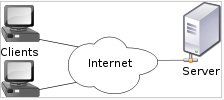
\includegraphics[width=13cm]{images/client-server.PNG}
		\caption{Server Diagram}
		\label{fig:form}
	\end{figure}

	\subsection{Хэрэглэгч болон Серверийн topology диаграмм}	

	\begin{figure}
		\centering
		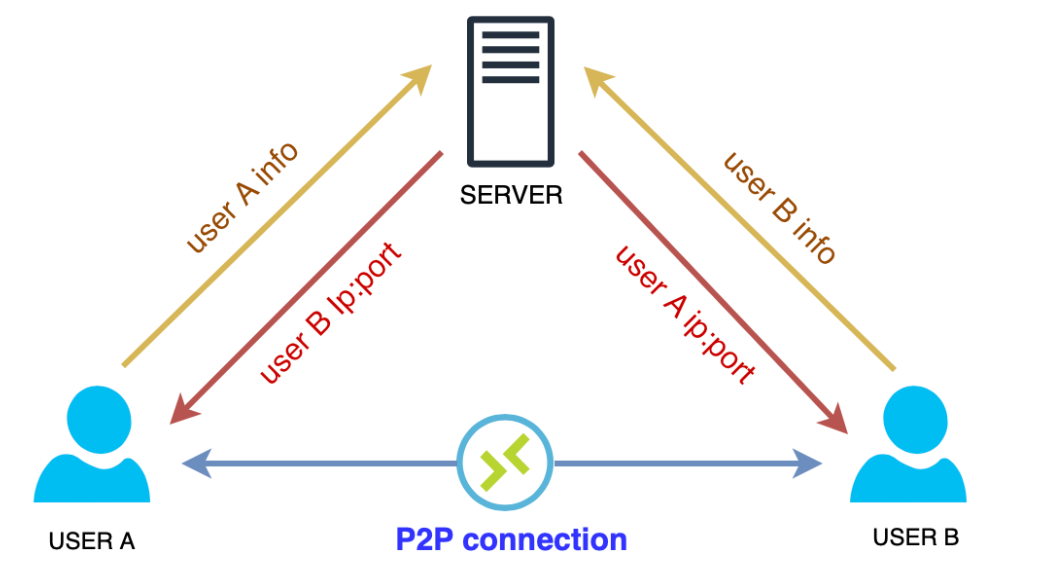
\includegraphics[width=15cm]{images/diagram.png}
		\caption{Connection Diagram}
		\label{fig:form}
	\end{figure}
	\pagebreak

